
\documentclass[UTF8]{ctexart}
\usepackage{lmodern}
\usepackage{amsmath}
\usepackage{amssymb}
\usepackage{graphicx}
\usepackage{xcolor}
\usepackage{geometry}
\usepackage{tikz}
\usepackage{caption}
\usepackage{float}
\usepackage{pgfplots}
\usepackage{mathtools}
\geometry{left=2.18cm,right=2.18cm,top=1.54cm,bottom=2.0cm}
\pagestyle{empty}
\pgfplotsset{compat=1.18}
\title{\textbf {2025春计算方法--实验报告 \#3}}
\author{姓名:\underline{~~~~~~~~~~~}  学号:\underline{~~~~~~~~~~~~~~~~~} }
\date{\today}


\begin{document}


\maketitle

运行环境:\underline{~~~~~~~~~~~~}

\section*{实验内容与要求}


分别编写 Newton 迭代法 (通常也称 Newton-Raphson 迭代法)
\[\color{blue}x_{n+1}=x_n-\frac{f(x_n)}{f'(x_n)}\]
和霍氏迭代法
 \[\color{blue} x_{n+1}= x_n - \frac{2f(x_n)f'(x_n)}{2f'(x_n)f'(x_n) - f(x_n)f''(x_n)}, \, n=0,1,2,\cdots\]
的通用程序, 并利用它们对如下非线性方程
\[\color{blue} f(x)\coloneqq{\arctan(x)}+0.2x\sin\left(\dfrac x2\right)+0.601958 =0\]
求根,计算中的停止条件为$\color{blue}|f(x_n)|<10^{-8}$或迭代步数~$\color{blue}n>10^4$(可视为迭代失败).
\textbf{提示}:编程前分别手算出$~\color{blue}f'(x), f''(x)$。

\begin{itemize}
    \item 列表给出两种迭代方法在初始点 $x_0$ 依次取值$-75, -60,-50, -40, -30, -20, -10, -5, 0, 6, 15, 25, 35,$ $ 45, 50, 60, 75$时的迭代步数(若迭代步数超过1万步,可视为迭代失败)以及相应的数值解~$x_n$~(保留小数点后6位; 迭代失败时无需给出);
    \item 比较并分析两种方法的优劣,给出合理的算法分析并作实验小结。
\end{itemize}

\begin{figure}[H]
    \begin{center}
        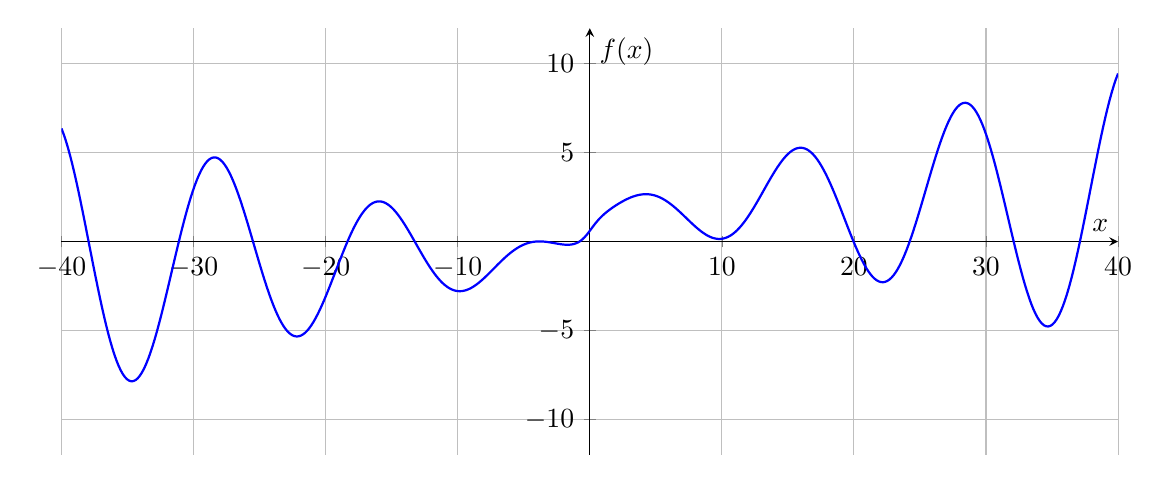
\begin{tikzpicture}
            \begin{axis}[
              xlabel={$x$},
              ylabel={$f(x)$},
              domain=-40:40,
              samples=500,
              axis lines=middle,
              xmin=-40, xmax=40,
              ymin=-12, ymax=12,
              grid=both,
              width=15cm,
              height=7cm,
            ]
            \addplot[blue, thick] { (pi/180)*atan(x) + 0.2*x*sin(deg(x/2)) + 0.601958 };
            \end{axis}
        \end{tikzpicture}
        \caption{函数图像}
        \label{fig:fig1}
    \end{center}
\end{figure}


\clearpage

\section{数值结果(列表或作图)}
\begin{table}[H]
\centering
\caption{实验结果: 误差精度~$\varepsilon = 10^{-9}$, 最大迭代步数为$10^4$}\begin{tabular}{ccccc}
\hline
Newton步数 & 数值解 & \color{blue}{初始点} & 霍氏步数 & 数值解 \\
\hline
3  & -75.524836 & \color{blue}{-75} & 3  & -75.524836 \\
6  & -75.524836 & \color{blue}{-60} & 5  & -62.983302 \\
3  & -50.453858 & \color{blue}{-50} & 3  & -50.453858 \\
5  & -37.948118 & \color{blue}{-40} & 4  & -37.948118 \\
4  & -31.113718 & \color{blue}{-30} & 3  & -31.113718 \\
4  & -18.345832 & \color{blue}{-20} & 3  & -18.345832 \\
4  & -43.765725 & \color{blue}{-10} & 6  & -13.253998 \\
6  & -4.069180  & \color{blue}{-5}  & 4  & -4.069180 \\
5  & -0.777558  & \color{blue}{0}   & 3  & -0.777558 \\
53 & -138.299622& \color{blue}{6}   & 19 & -0.777558 \\
15 & 119.561796 & \color{blue}{15}  & 17 & 100.314946 \\
4  & 24.221546  & \color{blue}{25}  & 3  & 24.221546 \\
5  & 44.470662  & \color{blue}{35}  & 5  & 37.112548 \\
3  & 44.470662  & \color{blue}{45}  & 3  & 44.470662 \\
3  & 49.830044  & \color{blue}{50}  & 2  & 49.830044 \\
6  & 75.109719  & \color{blue}{60}  & 5  & 62.484953 \\
3  & 75.109719  & \color{blue}{75}  & 2  & 75.109719 \\
\hline
\end{tabular}
\label{tab:tab1}
\end{table}

{\textbf Newton得到的解可能与初值偏离较大,Halley法可以较好调节步长以避免这个问题。}

\section{算法分析}

从实验结果表格中,我们可以观察到以下几点:

\begin{itemize}
    \item \textbf{Newton 迭代法的收敛性}:Newton 迭代法在初始点较接近实际根的情况下,收敛速度非常快。由于 Newton 迭代法依赖于一阶导数,因此在函数 $f(x)$ 的一阶导数不为零或变化不剧烈的情况下,能够较快收敛到根。然而,当初始点较远或导数接近零时,Newton 迭代法可能会发生收敛缓慢或者发散的情况。
    \item \textbf{霍氏迭代法的表现}:霍氏迭代法引入了二阶导数的修正,因此在某些情况下比 Newton 迭代法更稳定,特别是在初始点较远或函数一阶导数变化剧烈时,霍氏迭代法表现出更好的适应性。霍氏迭代法在处理复杂的非线性方程时,通过二阶导数减少了迭代的振荡和不稳定性。
    \item \textbf{迭代步数的比较}:从迭代步数的统计来看,Newton 迭代法在初始点靠近根的情况下通常收敛更快,但当初始点较远时,霍氏迭代法的表现更为稳定。Newton 法更容易在初始点远离根时表现出发散或振荡行为,而霍氏法则更适合在导数变化剧烈的情况下使用。
\end{itemize}

\section{实验小结}

在本次数值实验中,我们分别测试了 Newton 迭代法和霍氏迭代法对非线性方程的求解表现。通过实验分析,我们得出以下结论:

\begin{itemize}
    \item \textbf{Newton 迭代法的优点}:Newton 迭代法的主要优点在于其快速收敛,尤其是在初始点接近根时。该方法在许多实际应用中因其简单且高效而广泛应用。
    \item \textbf{Newton 迭代法的缺点}:其缺点在于对初始点的敏感性较高,容易在函数的导数接近零时失效。此外,当初始点距离根较远时,Newton 迭代法容易发散,尤其是当函数具有多重根或复杂的非线性行为时。
    \item \textbf{霍氏迭代法的优点}:霍氏迭代法的主要优势在于其更好的稳定性,尤其是在初始点较远或函数导数变化较大的情况下表现更为优异。由于考虑了二阶导数的影响,它在处理复杂非线性方程时有更好的收敛性。
    \item \textbf{霍氏迭代法的缺点}:由于引入了二阶导数,霍氏迭代法的计算量相比 Newton 法有所增加,这可能在每次迭代的成本上增加一定的计算复杂度。此外,当二阶导数较小或为零时,霍氏法的效果可能不如预期。
\end{itemize}

总的来说,Newton 迭代法更适用于初始点较接近根且导数变化平缓的情况,而霍氏迭代法在处理复杂非线性方程时表现出更好的适应性。通过对两种方法的比较,我们可以根据不同的实际问题选择合适的求根方法,以提高计算效率和收敛速度。


\end{document}
